\chapter{Estudo de Caso}
\label{estudodecaso}

Estudo de caso é uma metodologia de pesquisa adequada para estudar fenômenos contemporâneos em seu contexto natural \cite{runeson}. Com base nessa afirmação e na necessidade de avaliar o modelo proposto neste trabalho e sua utilização, foi realizado um estudo de caso no Laboratório de Sistemas Embarcados e Computação Pervasiva (Embedded Lab)\footnote{\url{http://www.embeddedlab.org/}}. O Embedded Lab está localizado na UFCG e foi escolhido em virtude das suas relações envolvendo a academia e a indústria.

Vários projetos são executados no Embedded Lab em parceria com empresas, com o objetivo de desenvolver produtos de \textit{software}. Em todos os projetos do Embedded Lab com foco em desenvolvimento de \textit{software}, a metodologia para gestão e planejamento utilizada é o \textit{Scrum}. Portanto, o contexto no qual este estudo de caso foi realizado é o da indústria, com utilização de \textit{Scrum} como metodologia ágil adotada. Assim, os resultados e conclusões obtidos neste estudo de caso são referentes a esse contexto. O estudo de caso foi realizado em três projetos, onde cada um deles foi considerado uma unidade de análise. {\color{red} A duração foi de X dias.}

\section{\textit{Design} do Estudo de Caso}
\label{estudodecaso:design}

\subsection{Objetivos}
\label{estudodecaso:design:objetivos}

Para este estudo de caso, foram definidos dois principais objetivos:

\begin{enumerate}
  \item Verificar a fidelidade do modelo proposto para a avaliação do TE de equipes \textit{Scrum} com relação ao mundo real;
  \item Verificar a utilidade da abordagem para utilização do modelo em projetos \textit{Scrum}.
\end{enumerate}

\subsection{Objetos de Estudo}
\label{estudodecaso:design:objetos}

Os objetos de estudo são:

\begin{enumerate}
  \item O modelo proposto para representar o TE de equipes \textit{Scrum};
  \item A abordagem proposta para utilização do modelo.
\end{enumerate}

Logo, com base nos objetos de estudo definidos, deseja-se avaliar: a precisão do modelo proposto, a sua utilidade para auxiliar na liderança de equipes \textit{Scrum} e a facilidade de implementação e utilização da abordagem proposta.

\subsection{Questões de Pesquisa}
\label{estudodecaso:design:perguntas}

Com base nos objetivos definidos para este estudo de caso e visando alcançá-los, foram definidas as seguintes questões de pesquisa:

\begin{itemize}
  \item \textit{PP1}: O modelo proposto mensura de forma precisa o TE de equipes Scrum?
  \item \textit{PP2}: A utilização do modelo auxília na detecção de oportunidades de melhoria do TE de equipes Scrum?
  \item \textit{PP3}: A abordagem proposta é de fácil implementação e utilização?
  \item \textit{PP4}: O custo-benefício de utilizar a abordagem é positivo?
\end{itemize}

Dadas as questões de pesquisa definidas acima, as seguintes hipóteses foram definidas para respondê-las:

\begin{itemize}
  \item \textit{H0-1}: O modelo proposto não mensura de forma precisa o TE de equipes Scrum;
  \item \textit{HA-1}: O modelo proposto mensura de forma precisa o TE de equipes Scrum;
  \item \textit{H0-2}: A utilização do modelo não auxilia na detecção de oportunidades de melhoria do TE de equipes Scrum;
  \item \textit{HA-2}: A utilização do modelo auxilia na detecção de oportunidades de melhoria do TE de equipes Scrum;
  \item \textit{H0-3}: A abordagem proposta não é de fácil implementação e utilização;
  \item \textit{HA-3}: A abordagem proposta é de fácil implementação e utilização;
  \item \textit{H0-4}: O custo-benefício de utilizar a abordagem não é positivo;
  \item \textit{HA-4}: O custo-benefício de utilizar a abordagem é positivo.
\end{itemize}

Assim, \textit{H0-1} e \textit{HA-1} estão relacionadas à \textit{PP1}, \textit{H0-2} e \textit{HA-2} estão relacionadas à \textit{PP2}, \textit{H0-3} e \textit{HA-3} estão relacionadas à \textit{PP3}, e \textit{H0-4} e \textit{HA-4} estão relacionadas à \textit{PP4}.

\subsection{Unidades de Análise}
\label{estudodecaso:design:unidades}

Este estudo de caso foi realizado em três unidades de análise. Cada unidade análise corresponde a um projeto de desenvolvimento de \textit{software} sendo executado no Embedded Lab. Essas unidades de análise foram nomeadas de Projeto A, Projeto B e Projeto C.

A equipe do Projeto A está trabalhando no desenvolvimento de um aplicativo para Desktop/Tablet x(86), Windows 8-10. Para o desenvolvimento desse projeto estão sendo utilizadas as tecnologias .NET, C\# e NUnit, além da Visual Studio (com ReSharper) como IDE (\textit{Integrated Development Environment}). De acordo com o \textit{Scrum Master} desse projeto, o escopo da aplicação sendo desenvolvida é relativamente simples, mas a diversidade das plataformas suportadas aumenta a sua complexidade. Contudo, inicialmente o cronograma inicial do projeto era tranquilo, mas a realocação de alguns membros da equipe para dar suporte a um projeto anterior tem dificultado o cumprimento do cronograma.

O aplicativo desenvolvido no Projeto B é uma ferramenta para monitoramento e controle de ativos de segurança patrimonial, e, de acordo com \textit{Scrum Master}, o escopo é complexo. Esse aplicativo está sendo desenvolvido para Android e utiliza as tecnologias SIP e RTSP. O cronograma inicial do projeto foi descrito como simples. Entretanto, a dependência de um \textit{Hardware} sendo desenvolvido por outra entidade pode afetar o cumprimento desse cronograma.

A equipe do Projeto C está desenvolvendo um aplicativo \textit{web}, utilizando Django e Python. O produto final depende da integração de outros componentes de \textit{Software} e \textit{Hardware} desenvolvidos por outros projetos do Embedded Lab e também do cliente. De acordo com o \textit{Scrum Master}, o cronograma inicial estava sendo cumprido no prazo, mas houveram algumas mudanças de requisitos que podem comprometer o seu cumprimento.

Na Tabela \ref{estudodecaso:design:unidades:tabela}, há informações referentes aos membros das equipes das unidades de Análise.

\begin{table}[ht!]
\centering
\caption{Experiência das Equipes das Unidades de Análise.}
\label{estudodecaso:design:unidades:tabela}
\begin{tabular}{|l|c|c|c|}
\hline
\multicolumn{1}{|c|}{}                                                                                                                                               & \multicolumn{3}{c|}{\textbf{Projeto}} \\ \hline
\multicolumn{1}{|c|}{\textbf{Característica}}                                                                                                                        & \textbf{A}  & \textbf{B} & \textbf{C} \\ \hline
\begin{tabular}[c]{@{}l@{}}Experiência, em média de anos, dos integrantes da equipe participando\\ em projetos de desenvolvimento de \textit{software}.\end{tabular} & 2.5         & 2          & 2          \\ \hline
\begin{tabular}[c]{@{}l@{}}Experiência, em média de anos, dos integrantes da equipe trabalhando\\ em equipes ágeis.\end{tabular}                                     & 1           & 1          & 2          \\ \hline
\end{tabular}
\end{table}

\subsection{Sujeitos - Quem utiliza a abordagem e o modelo?}
\label{estudodecaso:design:sujeitos}

Para cada unidade de análise, os sujeitos que irão utilizar participar deste estudo de caso são líderes de projeto que atuam como \textit{Scrum Masters}. No Embedded Lab, esses sujeitos realizam atividades relacionadas ao processo e o gerenciamento da equipe, atividades relacionadas ao \textit{design} dos produtos, do ponto de vista gráfico e arquitetural de produto, além de implementação.

Na Tabela \ref{sujeitos}, são apresentados os perfis dos sujeitos em relação à experiência, em anos, desenvolvendo \textit{software}, liderando projetos de desenvolvimento, utilizando métricas no suporte à tomada de decisões e utilizando métodos ágeis.

\begin{table}[ht!]
\centering
\caption{Perfis dos Sujeitos.}
\label{sujeitos}
\resizebox{\textwidth}{!}{\begin{tabular}{|l|c|c|c|}
\hline
 & \multicolumn{3}{c|}{\textbf{Sujeito}} \\ \hline
\multicolumn{1}{|c|}{\textbf{Característica}}                                           & \textbf{1}  & \textbf{2} & \textbf{3} \\ \hline
Experiência, em anos, trabalhando em projetos de desenvolvimento de \textit{software}            & 5           & 10         & 10         \\ \hline
Experiência, em anos, liderando projetos de desenvolvimento de \textit{software}                 & 0.5         & 3          & 2          \\ \hline
Experiência, em anos, utilizando métricas e indicadores no suporte à tomada de decisões & 1.5         & 2          & 6          \\ \hline
Experiência, em anos, utilizando métodos ágeis                                          & 5           & 2          & 7          \\ \hline
\end{tabular}}
\end{table}

\subsection{Métodos}
\label{estudodecaso:design:metodos}

A coleta de dados é uma atividade necessária para responder as questões de pesquisas de um estudo de caso experimental. De acordo com Lethbridge et al. \cite{lethbridge}, há três diferentes categorias de métodos para coleta de dados: direto (e.g., entrevistas), indireto (e.g., \textit{survey}) e independente (e.g., análise de documentação).

Neste estudo de caso, o processo de coleta de dados ocorrerá pelos métodos direto e indireto. Os dados referentes aos nós de entrada do modelo serão coletados em entrevistas. Por outro lado, os dados referentes à satisfação dos sujeitos e utilidade da abordagem e do modelo serão coletados por questionários.

\subsection{Procedimento}
\label{estudodecaso:design:procedimento}

Antes de iniciar este estudo caso, foi realizada a definição do modelo, das perguntas para alimentação dos nós de entrada e dos questionários para avaliação do modelo e da abordagen. Para efetuar os cálculos do modelo, foi utilizada a ferramenta AgenaRisk. Em virtude de algumas limitações com licensas da ferramenta, o modelo foi criado e todos os cálculos realizados na máquina do pesquisador. Após a obtenção dos resultados, eles foram apresentados aos sujeitos pelo pesquisador.

Com base no que foi definido acima, este estudo de caso foi dividido em duas fases: \textit{Treinamento} e \textit{Utilização da Abordagem}.

\subsubsection{Fase 1 - Treinamento}
\label{estudodecaso:design:procedimento:treinamento}

O objetivo desta fase do estudo de caso é prover aos sujeitos o entendimento dos conceitos relacionados aos objetos de estudo. Assim, espera-se que ao final dessa fase qualquer dúvida em relação à esses fatores seja sanada para que os resultados não sejam influenciados por má-interpretação das perguntas das entrevistas e dos questionários.

À princípio, os conceitos de Redes Bayesianas, Nós Ranqueados, além de \textit{Funções de Probabilidade}, suas aplicações e funcionamento foram explicados para facilitar o entendimento da construção do modelo. Após isso, o modelo proposto nesta dissertação, e os relacionamentos entre os fatores que o compõem, foram explicados. Em seguida, foi explicado como seria realizado o processo de coleta de dados e quais perguntas do Apêndice \ref{questionarios} são referentes à quais nós de entrada do modelo. Por fim, foi explicado como é feita a análise dos resultados gerados pelo modelo, e como é possível identificar oportunidades de melhoria no TE. Alguns exemplos foram utilizados nessa fase para auxiliar no entendimento dos sujeitos.

\subsubsection{Fase 2 - Utilização da Abordagem}
\label{estudodecaso:design:procedimento:abordagem}

{\color{red} Utilização da abordagem...}

\subsection{Ameaças à Validade}
\label{estudodecaso:design:ameacas}

Runeson et al. \cite{runeson} afirmam que há diferentes maneiras de classificar aspectos da validade e ameaças à validade na literatura. No trabalho anteriormente citado, eles definem um esquema de classificação que distingue bem quatro aspectos da validade de um estudo de caso. São eles: \textit{Validade de Construção}, \textit{Validade Interna}, \textit{Validade Externa e Confiabilidade}.

O aspecto da \textit{Validade de Construção} está relacionado com o fato de o que é estudado realmente representar o que o pesquisador tem em mente estar de acordo com as questões de pesquisa. Por exemplo, o assunto abordado nas entrevistas é interpretado pelos pesquisador e os entrevistados da maneira diferente. Portanto, neste estudo de caso, apesar do treinamento realizado para os sujeitos envolvidos, há a possibilidade deles interpretarem as perguntas dos questionários de tal forma que não condiz com os objetivos para os quais elas foram elaboradas.

A \textit{Validade Interna} diz respeito ao ato de verificar se um determinado fator afeta o fator investigado, quando há o risco de um terceiro fator que influenciar o fator investigado. Logo, como neste estudo de caso adotou-se o TE como indicador do desempenho da equipe, e há outros fatores como FATOR A, FATOR B e FATOR C que influenciam o desempenho da equipe \cite{}, também há ameaças à \textit{Validade Interna deste estudo}.

Com relação ao aspecto da \textit{Validade Externa}, que está relacionado em saber até que ponto é possível generalizar os resultados, e em que medida os resultados são de interesse para outras pessoas fora do caso investigado. Durante a análise da \textit{Validade Externa}, o pesquisador precisa analisar se os resultados podem ser relevantes para outros casos. Portanto, como os objetos de estudo deste estudo de caso foram avaliados para apenas três unidades de análise, a generealização dos resultados para todas as equipes \textit{Scrum} do mundo não é possível.

Além desses aspectos, também há a \textit{Confiabilidade}, que está relacionada à dependência dos dados coletados e sua análise em relação ao pesquisador. Assim, como é necessário que os sujeitos deste estudo de caso respondam questionários com o intuito de poder avaliar as equipes que estão sendo lideradas por eles, há o risco de haver viés nos dados coletados. Isso pode acontecer não apenas pelo fato dos sujeitos estarem envolvidos com suas equipes e o seu trabalho, mas também pela possibilidade das perguntas não serem claras o suficiente para facilitar a sua resposta. Também há a possibilidade das perguntas do questionário de satisfação não terem sido bem elaboradas. Além disso, este estudo de caso foi conduzido apenas com equipes \textit{Scrum}, uma dentre as várias metodologias ágeis existentes. Logo, esses fatores também afetam a \textit{Confiabilidade} deste estudo de caso.

\section{Coleta dos Dados}
\label{estudodecaso:coleta}

Como forma de alimentar os nós de entrada do modelo, foram elaboradas perguntas simples e diretas, visando diminuir o tempo necessário para respondê-las. Para cada nó de entrada do modelo, foi elaborada uma pergunta, e suas respostas são todas objetivas, de única escolha, na seguinta escala: Falso, Mais Falso que Verdadeiro, Nem Verdadeiro nem Falso, Mais Verdadeiro que Falso e Verdadeiro. Essa escala foi adotada com base na escala que é utilizada no \textit{survey online} ferramenta \textit{Comparative Agility}. Além dos dados para alimentação dos nós, perguntas relacionadas às métricas para o cálculo da eficiência das equipes também foram inseridas nesse questionário. Essas perguntas estão definidas no Apêndice \ref{questionarios}.

A coleta de dados necessária para responder as perguntas de pesquisa deste estudo de caso foi feita com a utilização de um questionário, no formato de formulário \textit{online}. Dessa forma, os sujeitos podem respondê-lo quando acharem cômodo, de modo que não venha a incomodar em sua rotina de trabalho. Para a criação desses questionários, foi decidido utilizar o Google Forms\footnote{\url{https://www.google.com/forms/about/}}, ferramenta que permite criar questionários e armazenar os dados coletados neles em planilhas providas pela ferramenta Google Sheets\footnote{\url{https://www.google.com/sheets/about/}}. Além de permitir criar os questionários e armazenar os resultados, essas ferramentas também facilitam o compartilhamento de ambos, com a utilização de links.

O questionário referente às perguntas de pesquisa deste estudo de caso contém perguntas diretas, que seguem o mesmo padrão das perguntas elaboradas para alimentar os nós de entrada do modelo. Contudo, também há a oportunidade de inserção de texto puro, onde os sujeitos podem comentar e dar mais opiniões à respeito da pergunta de pesquisa tratada.

As perguntas definidas para responder as perguntas de pesquisa deste estuda de caso estão definidas no Apêndice \ref{satisfacao}. Portanto, a pergunta de pesquisa \textit{PP1} é respondida com base nas respostas das perguntas 1 e 2 desse Apêndice. A pergunta de pesquisa \textit{PP2} é respondida de acordo com as respostas das perguntas 3 e 4. As perguntas 5 e 6 do Apêndice \ref{satisfacao} são referentes à pergunta de pesquisa \textit{PP3}. Finalmente, a pergunta de pesquisa \textit{PP4} é respondida de acordo com as perguntas 7 e 8 desse Apêndice.

\section{Análise dos Dados}
\label{estudodecaso:analise}

Para responder as perguntas de pesquisa definidas neste estudo de caso, a análise é realizada com base nas respostas das perguntas objetivas definidas no Apêndice \ref{satisfacao}. Como cada pergunta objetiva pode ser respondida em um escala de 5 pontos, decidiu-se mapear as possíveis respostas dessas perguntas da seguinte forma:

\begin{itemize}
  \item \textit{Falso}$\,\to\,1$
  \item \textit{Mais Falso que Verdadeiro}$\,\to\,2$
  \item \textit{Nem Verdadeiro nem Falso}$\,\to\,3$
  \item \textit{Mais Verdadeiro que Falso}$\,\to\,4$
  \item \textit{Verdadeiro}$\,\to\,5$
\end{itemize}

Dessa forma, é possível realizar uma análise mais objetiva utilizando métodos estatísticos.

\subsubsection{\textit{PP1}: O modelo proposto mensura de forma precisa o TE de equipes Scrum?}

Essa pergunta está relacionada à fidelidade dos resultados calculados pelo modelo em relação ao cenário em que esses cálculos. Baseado na eficiência da equipe, e considerando outros fatores externos que podem influenciar essa eficiência, os \textit{Scrum Masters} avaliaram se a qualidade do TE calculada pelo modelo condiz com o cenário em que foi avaliado.

Para responder essa pergunta de pesquisa, foi necessário avaliar as hipótestes \textit{H0-1} e \textit{HA-1}. Como a pergunta 1 do questionário de satisfação (i.e., Apêndice \ref{satisfacao}) corresponde à pergunta de pesquisa \textit{PP1}, foi definida a seguinte condição:

Caso $v_{q1B} \le 3$, onde $v_{q1B}$ representa a média das respostas para \textit{PP1}, deve-se aceitar \textit{H0-1}. Caso contrário, rejeita-se \textit{H0-1} e, consequentemente, assume-se que \textit{HA-1} é verdadeira.

\subsubsection{\textit{PP2}: A utilização do modelo auxília na detecção de oportunidades de melhoria do TE de equipes Scrum?}

Para responder essa pergunta, foi necessário avaliar as hipóteses \textit{H0-2} e \textit{HA-2}. Assim, baseado na pergunta 3 do questionário, que corresponde à pergunta de pesquisa \textit{PP2}, foi definida a seguinte condição:

Caso $v_{q3B} \le 3$, onde $v_{q3B}$ representa a média das respostas para \textit{PP2}, deve-se aceitar \textit{H0-2}. Caso contrário, rejeita-se \textit{H0-2} e, consequentemente, assume-se que \textit{HA-2} é verdadeira.

\subsubsection{\textit{PP3}: A abordagem proposta é de fácil implementação e utilização?}

É necessário avaliar as hipóteses \textit{H0-3} e \textit{HA-3} para responder essa pergunta. Assim, como a pergunta 5 do questionário de satisfação está relacionada à pergunta de pesquisa \textit{PP3}, foi definida a seguinte condição:

Caso $v_{q5B} \le 3$, onde $v_{q5B}$ representa a média das respostas para \textit{PP3}, deve-se aceitar \textit{H0-3}. Caso contrário, rejeita-se \textit{H0-3} e, consequentemente, assume-se que \textit{HA-3} é verdadeira.

\subsubsection{\textit{PP4}: O custo-benefício de utilizar a abordagem é positivo?}

De forma análoga às perguntas de pesquisa anteriores, para responder essa pergunta, é necessário avaliar as hipóteses \textit{H0-4} e \textit{HA-4}. Portanto, baseado na pergunta 7 do questionário, que corresponde à pergunta de pesquisa \textit{PP4}, foi definida a seguinte condição:

Caso $v_{q7B} \le 3$, onde $v_{q7B}$ representa a média das respostas para \textit{PP4}, deve-se aceitar \textit{H0-4}. Caso contrário, rejeita-se \textit{H0-4} e, consequentemente, assume-se que \textit{HA-4} é verdadeira.

\section{Resultados}
\label{estudodecaso:resultados}

Para responder as perguntas de pesquisa deste estudo de caso, os sujeitos utilizaram a abordagem e o modelo propostos neste trabalho para avaliar o TE de suas equipes em três \textit{Sprints}. As Figuras \ref{estudodecaso:resultados:projetoA}, \ref{estudodecaso:resultados:projetoB} e \ref{estudodecaso:resultados:projetoC} contém os resultados calculados pelo modelo para as equipes das três unidades de análise definidas. 

\begin{figure}[ht!]
\begin{center}
		\fbox{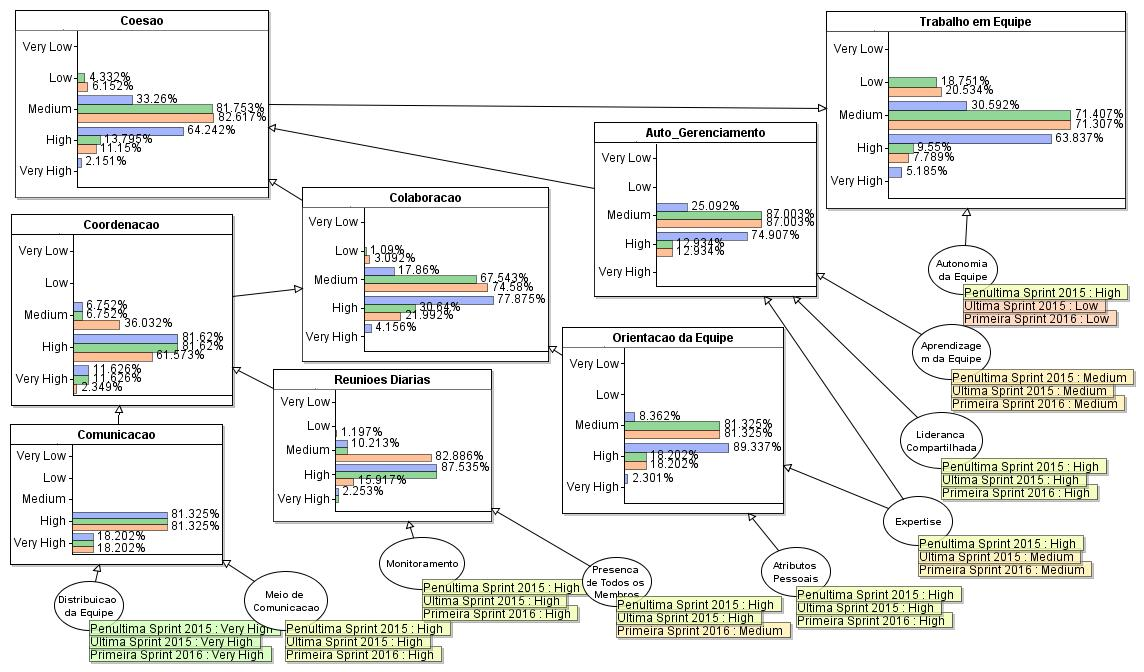
\includegraphics[scale=0.52]{resultados/resultadosProjetoA.jpg}}
	\end{center}
	\caption{Resultados Calculados pelo Modelo para o Projeto A.}
	\label{estudodecaso:resultados:projetoA}
\end{figure}

\begin{figure}[ht!]
\begin{center}
		\fbox{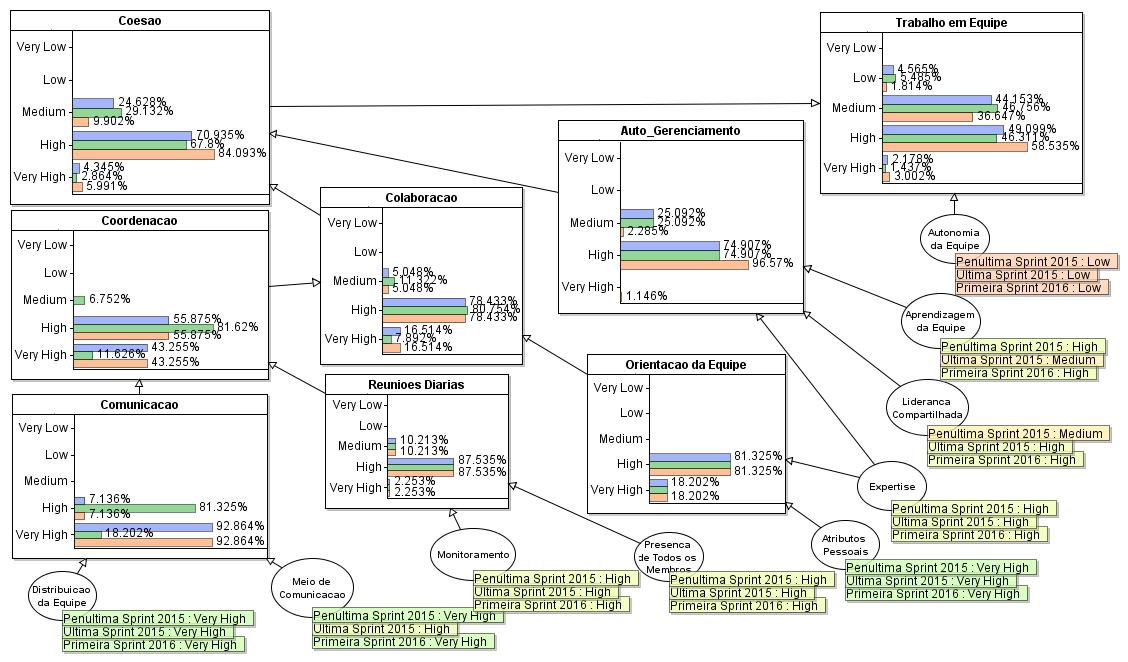
\includegraphics[scale=0.52]{resultados/resultadosProjetoB.jpg}}
	\end{center}
	\caption{Resultados Calculados pelo Modelo para o Projeto B.}
	\label{estudodecaso:resultados:projetoB}
\end{figure}

\begin{figure}[ht!]
\begin{center}
		\fbox{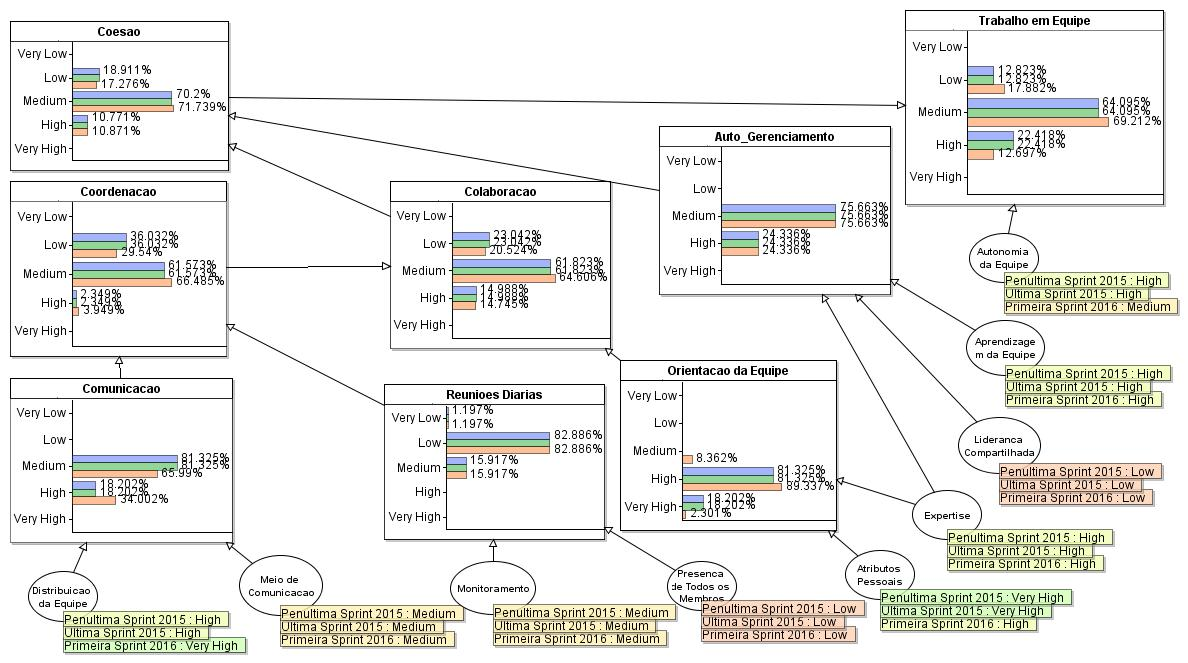
\includegraphics[scale=0.52]{resultados/resultadosProjetoC.jpg}}
	\end{center}
	\caption{Resultados Calculados pelo Modelo para o Projeto C.}
	\label{estudodecaso:resultados:projetoC}
\end{figure}

Contudo, os sujeitos precisaram analisar os resultados calculados pelo modelo, comparando-os com a eficiência de sua equipe, mas levando em consideração outros fatores que influenciam essa eficiência. A Tabela \ref{estudodecaso:resultados:eficiencias} contém a eficiência de cada equipe, em cada uma das \textit{sprints}, de acordo com os dados coletados.

\begin{table}[ht!]
\centering
\caption{Eficiência das Equipes nas três \textit{Sprints}.}
\label{estudodecaso:resultados:eficiencias}
\begin{tabular}{|l|c|c|c|}
\hline
\multicolumn{1}{|c|}{}                         & \multicolumn{3}{c|}{\textbf{Projeto}} \\ \hline
\multicolumn{1}{|c|}{\textbf{\textit{Sprint}}} & \textbf{A}  & \textbf{B} & \textbf{C} \\ \hline
Penúltima \textit{Sprint} de 2015              & 98,61\%     & 95,23\%    & 73,33\%    \\ \hline
Última \textit{Sprint} de 2015                 & 69,23\%     & 100\%      & 100\%      \\ \hline
Primeira \textit{Sprint} de 2016               & 70,51\%     & 100\%      & 77,77\%    \\ \hline
\end{tabular}
\end{table}

Após o término das três \textit{sprints}, com base nesses resultados, os sujeitos responderam o questionário de satisfação para avaliar a fidelidade do modelo; o seu auxílio na detecção de oportunidades de melhoria do TE; a facilidade para implementar e utilizar a abordagem proposta; e o custo-benefício de sua utilização.

As Figuras \ref{estudodecaso:resultados:fidelidade}, \ref{estudodecaso:resultados:auxilio}, \ref{estudodecaso:resultados:utilizacao} e \ref{estudodecaso:resultados:custoBeneficio} contém os resultados referentes às perguntas de pesquisa. Com base nesses resultados, é possível avaliar as hipóteses definidas para cada uma das perguntas de pesquisa.

\begin{figure}[ht!]
\begin{center}
		\fbox{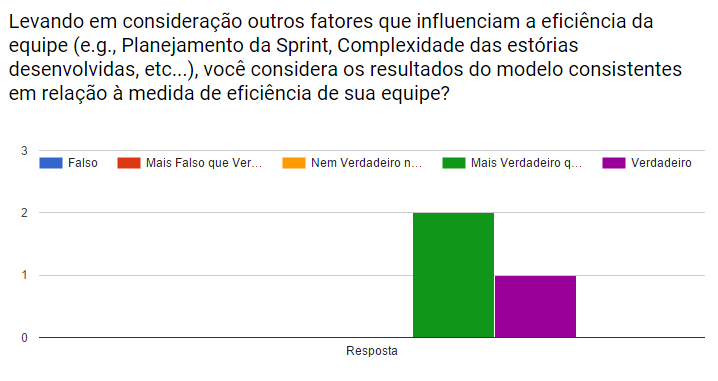
\includegraphics[scale=0.8]{resultados/fidelidade.png}}
	\end{center}
	\caption{Respostas para a Pergunta de Pesquisa \textit{PP1}.}
	\label{estudodecaso:resultados:fidelidade}
\end{figure}

\begin{figure}[ht!]
\begin{center}
		\fbox{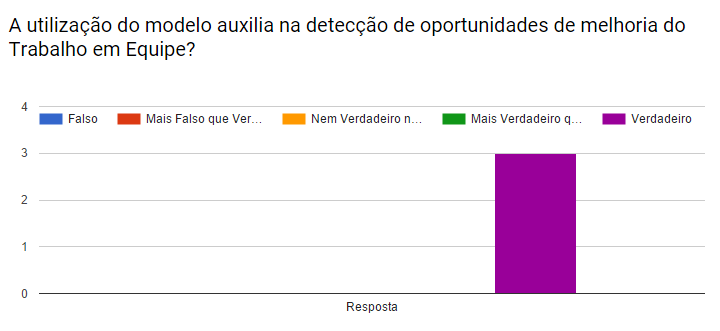
\includegraphics[scale=0.8]{resultados/auxilio.png}}
	\end{center}
	\caption{Respostas para a Pergunta de Pesquisa \textit{PP2}.}
	\label{estudodecaso:resultados:auxilio}
\end{figure}

\begin{figure}[ht!]
\begin{center}
		\fbox{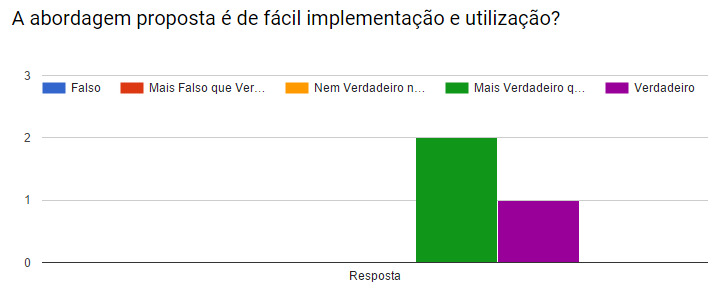
\includegraphics[scale=0.8]{resultados/utilizacao.png}}
	\end{center}
	\caption{Respostas para a Pergunta de Pesquisa \textit{PP3}.}
	\label{estudodecaso:resultados:utilizacao}
\end{figure}

\begin{figure}[ht!]
\begin{center}
		\fbox{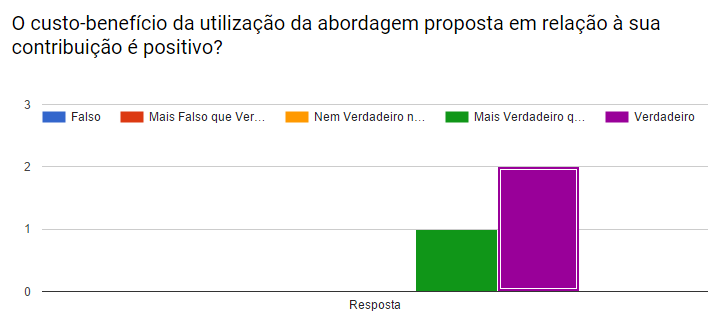
\includegraphics[scale=0.8]{resultados/custoBeneficio.png}}
	\end{center}
	\caption{Respostas para a Pergunta de Pesquisa \textit{PP4}.}
	\label{estudodecaso:resultados:custoBeneficio}
\end{figure}

De possse desses resultados, as hipóteses referentes às perguntas de pesquisa foram avaliadas. Todas as hipóteses foram avaliadas com o teste estatístico X, com nível de confiança de 95\%. Para as hipóteses \textit{H0-1}, \textit{H0-2}, \textit{H0-3} e \textit{H0-4}, os valores de $p$ obtidos foram A, B, C e D, respectivamente. Portanto, todas as hipóteses nulas foram rejeitadas. Consequentemente, as hipóteses alternativas (i.e., \textit{HA-1}, \textit{HA-2}, \textit{HA-3} e \textit{HA-4}) foram aceitas. Logo, todas as perguntas de pesquisa foram respondidas de forma positivamente. Assim, pode-se concluir que:

\begin{itemize}
  \item O modelo proposto mensura de forma precisa o TE de equipes Scrum;
  \item A utilização do modelo auxília na detecção de oportunidades de melhoria do TE de equipes Scrum;
  \item A abordagem proposta é de fácil implementação e utilização;
  \item O custo-benefício de utilizar a abordagem é positivo.
\end{itemize}

Além dessas respostas objetivas, os sujeitos também responderam de as perguntas 2, 4 e 6 do questionário de satisfação (Tabela \ref{satisfacao:tabela}), para prover mais informações à respeito do contexto das \textit{sprints} e externar seus pontos de vista de forma descritiva. As Figuras \ref{estudodecaso:resultados:respostasFidelidade}, \ref{estudodecaso:resultados:respostasAuxilio}, \ref{estudodecaso:resultados:respostasUtilizacao} contém, respectivamente, as respostas referentes às perguntas 2, 4 e 6 do questionário de satisfação.

\begin{figure}[ht!]
\begin{center}
		\fbox{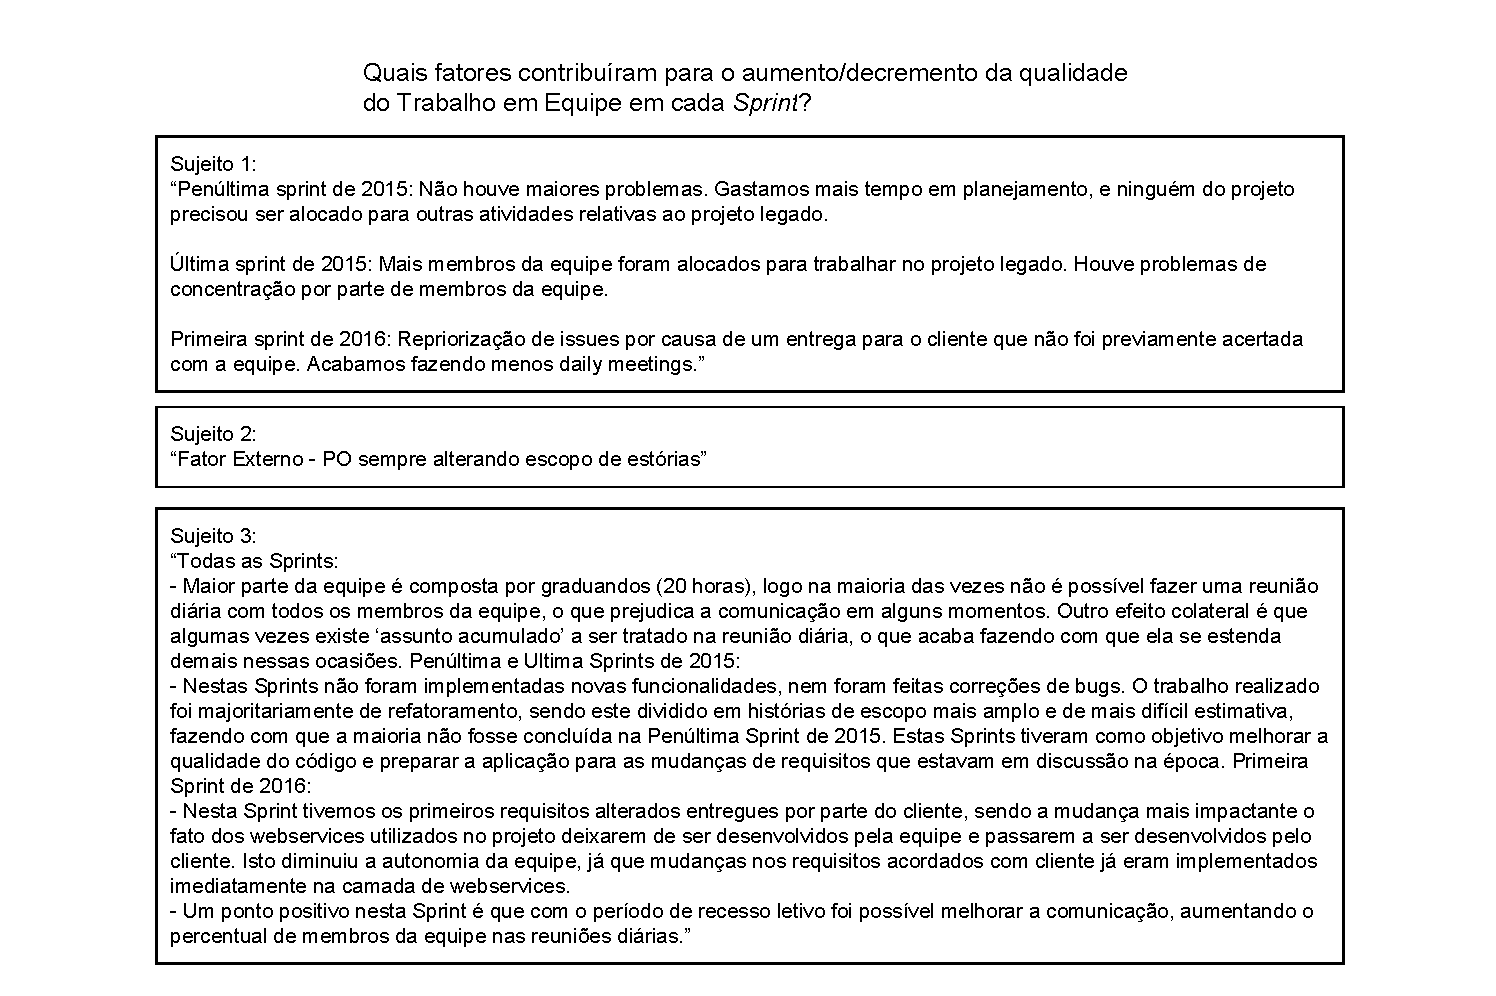
\includegraphics[scale=0.65]{resultados/fidelidade.pdf}}
	\end{center}
	\caption{Respostas para a Pergunta 2 do Questionário de Satisfação}
	\label{estudodecaso:resultados:respostasFidelidade}
\end{figure}

\begin{figure}[ht!]
\begin{center}
		\fbox{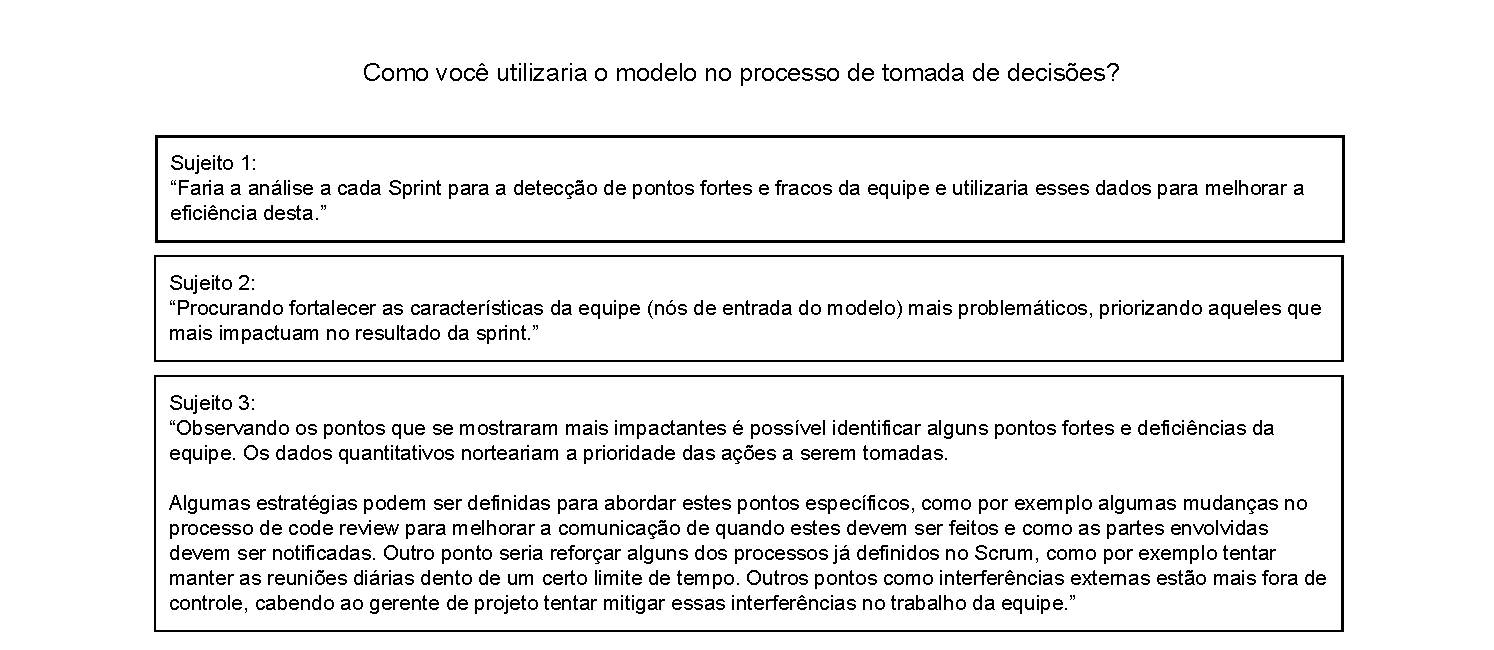
\includegraphics[scale=0.65]{resultados/auxilio.pdf}}
	\end{center}
	\caption{Respostas para a Pergunta 4 do Questionário de Satisfação}
	\label{estudodecaso:resultados:respostasAuxilio}
\end{figure}

\begin{figure}[ht!]
\begin{center}
		\fbox{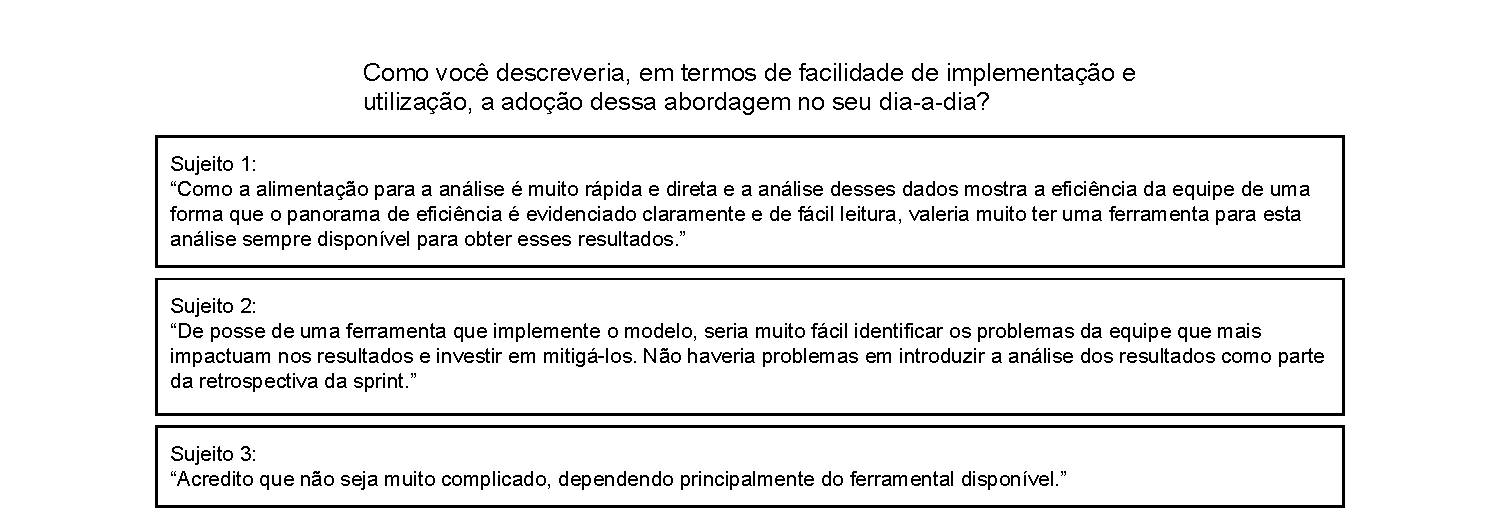
\includegraphics[scale=0.65]{resultados/utilizacao.pdf}}
	\end{center}
	\caption{Respostas para a Pergunta 6 do Questionário de Satisfação}
	\label{estudodecaso:resultados:respostasUtilizacao}
\end{figure}